\setcounter{exo}{0}

On donne les équations du moteur à courant continu :
\begin{itemize}
\item $u(t) = e(t)+ Ri(t) +L \dfrac{\text{d}i(t)}{\text{d} t}$;
\item $e(t)=K\omega(t)$;
\item $c(t)=Ki(t)$;
\item $c(t)-c_r(t) - f\omega(t)=J\dfrac{\text{d}\omega(t)}{\text{d} t}$.
\end{itemize}
\subparagraph{}
\textit{Réaliser le schéma-blocs.}

\ifprof
\begin{corrige}
\begin{center}
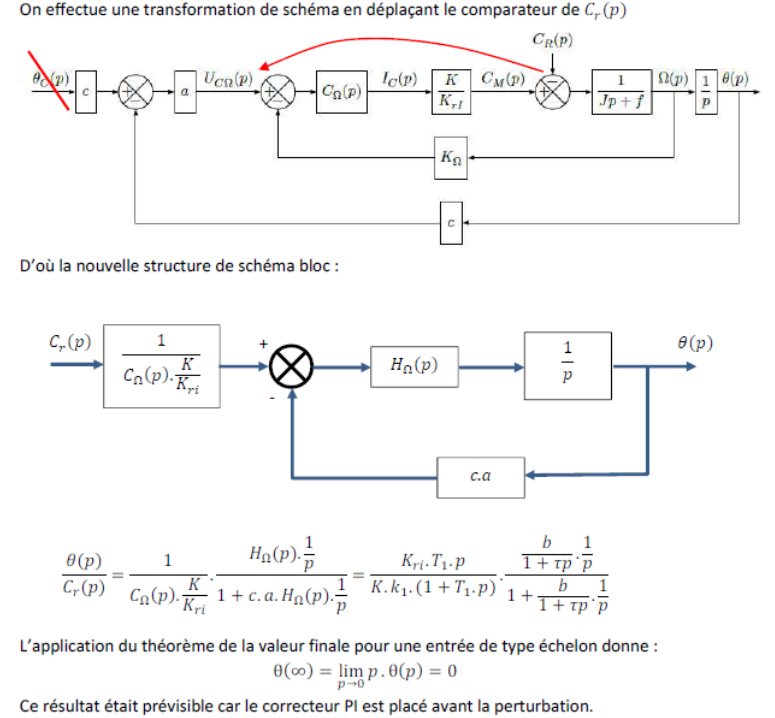
\includegraphics[width=.9\linewidth]{cor_01}
\end{center}
\end{corrige}
\else
\fi

\subsection*{Analyse de la fonction technique << mettre le tube sous pression >>.}


\ifprof
\else
Un schéma hydraulique simplifié est donné figure suivante.
\begin{center}
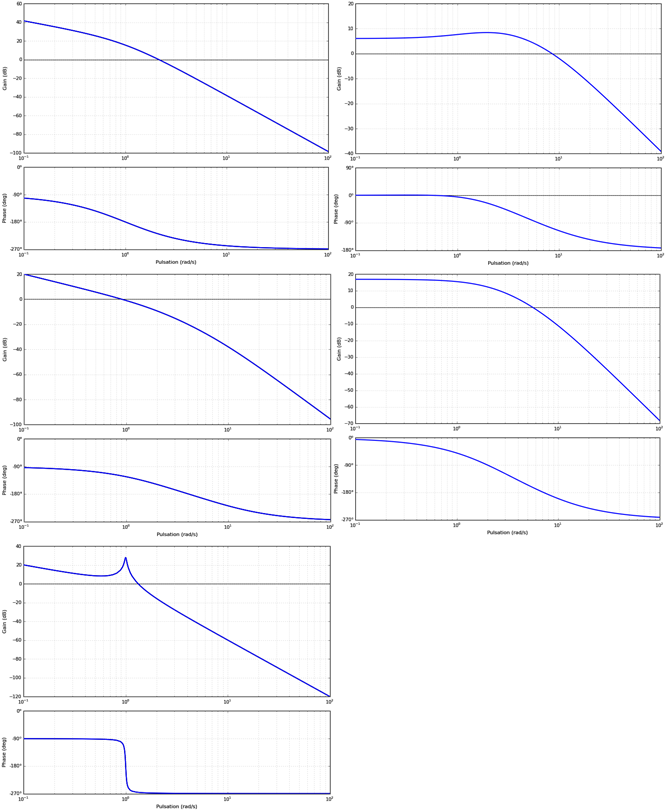
\includegraphics[width=\linewidth]{fig_01}

\end{center}
\fi

\subsection*{Mise en place du modèle}

En appliquant le théorème de la résultante dynamique selon $\vect{z}$ sur le piston du multiplicateur, on a : 
$
M\ddot{z}(t)=S_hp_h(t)-S_ep_e(t)-Mg-f\dot{z}(t).
$
\subparagraph{}
\textit{Déduire de la relation précédente l’équation reliant $Z(p)$, $P_e(p)$, $P_h(p)$, et $\text{Poids}(p)=Mg/p$, transformées de Laplace de $z(t)$, $P_e(t)$, $P_h(t)$ et du poids perçu comme une perturbation. Les conditions initiales sont supposées nulles.}
\ifprof
\begin{corrige}
$Mp^2 Z(p))=S_hP_h(p)-S_eP_e(pt)-\dfrac{Mg}{p}-fpZ(p)$
\end{corrige}
\else
\fi

%\subsection*{Modélisation du chariot avant}



\ifprof
\else
%\begin{center}
%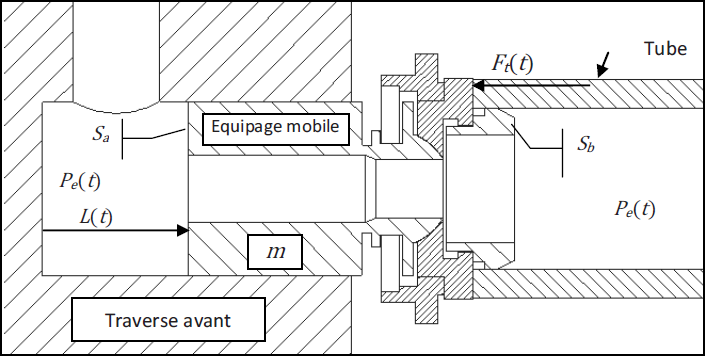
\includegraphics[width=.95\linewidth]{fig_03}
%\end{center}


On note :
\begin{itemize}
	\item $L(t)$ la position de l’équipage mobile repérée par rapport à sa position initiale;
	\item $V_t(t)$ le volume du tube;
	\item $F_t(t)$ l’effort du tube sur l’équipage mobile, avec $F_t(t) = - rL(t)$.
\end{itemize}

On néglige les variations de volume du tube dues à ses déformations. L’équation du débit s’écrit alors :
	$$Q_e (t)=(S_a-S_b ).\dfrac{\text{d}L(t)}{\text{d}t}+\dfrac{V_t}{B_e}  \dfrac{\text{d}P_e (t)}{\text{d}t}.$$


L’équation du mouvement de l’équipage mobile est donnée par : 
$$
m\ddot{L}(t)=-rL(t)+\left(S_a-S_b \right)p_e(t)-f'\dot{L}(t).
$$

\fi
\subparagraph{}
\textit{En déduire, en tenant compte de l’équation du débit, deux équations liant $L(p)$, $P_e(p)$ et $Q_e(p)$, transformées de Laplace de $L(t)$, $P_e(t)$ et $Q_e(t)$. }
\ifprof
\begin{corrige}
	$Q_e (p)=(S_a-S_b )p L(p)+\dfrac{V_t}{B_e}  p P_e(p)$
\end{corrige}
\else
\fi
Les conditions initiales sont supposées nulles.

\subparagraph{}
\textit{Compléter le schéma-blocs de l’ensemble (sans le distributeur hydraulique), l’entrée étant la pression d’huile régulée $P_r(p)$ et la sortie la pression d’épreuve dans le tube $P_e(p)$.}
\ifprof
\begin{corrige}
\end{corrige}
\else
\fi


\begin{center}
\rotatebox{90}{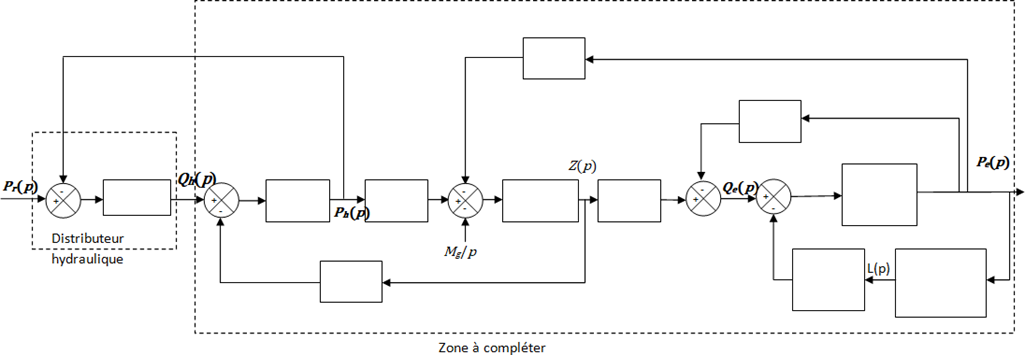
\includegraphics[height=.8\linewidth]{fig_10}}
\end{center}
